\documentclass{article}
\usepackage[utf8]{inputenc}
\usepackage{polski}
\usepackage[polish]{babel}
\usepackage{graphicx}    
\usepackage{caption}
\usepackage{subcaption}
\usepackage{epstopdf}
\usepackage{amsmath}
\usepackage{amsthm}
\usepackage{amsfonts}
\usepackage{hyperref}
\usepackage{url}
\usepackage{comment}
\usepackage{listings}
\usepackage{slashbox}
\usepackage{indentfirst}
\newtheorem{defi}{Definicja}
\newtheorem{twr}{Twierdzenie}
\newtheorem{alg}{Algorytm}
\setlength{\parindent}{15pt}
\lstset{numbers=left, numberstyle=\small, frame=L, xleftmargin=\parindent,}

\begin{document}
\title{\textbf{Analiza numeryczna (M) - pracownia 1 }\\ 
Implementacja i analiza metody obliczania logarytmu zaproponowanej w \cite{al-mohy11}\\}
\date{Wrocław, \today}
\author{Maksymilian Polarczyk\\ Prowadzący: Paweł Woźny}
\maketitle
\noindent Program zaimplementowano z wykorzystaniem języka \textbf{Julia}, w pliku \texttt{program.jl}. Wykresy zostały narysowane przy pomocy biblioteki \textbf{Plots} i razem z eksperymentami zamieszczone są w pliku \texttt{program.ipynb}.

\section{Wstęp}

	Awad H. Al-Mohy przedstawił w swojeje pracy\cite{al-mohy11} udoskonaloną pod względem numerycznym metodę Briggsa obliczania logarytmu dla liczb ze zbioru $\mathbb{C}\setminus\mathbb{R}^-$. Pierwotna metoda Henrego Briggsa opiera się na własności logarytmu $\log{x}=2\log{x^\frac{1}{2}}$ oraz przybliżeniu pierwszego rzędu $\log({1+x)} \approx x$, które jest dobre dla $x$ bliskich zera. Problem liczenia $\log{a}$ sprowadził więc, korzystając z powyższych własności, do problemu iteracyjnego liczenia wyrażenia ${2^k}log{(a^{1/2^{k}}-1)}$. Wadą tej metody jest podatność na zjawisko utraty cyfr znaczących w arytmetyce zmiennopozycyjnej podczas obliczania kluczowej wartości \begin{equation} \label{eq:briggs}	(a^{1/2^{k}}-1) \end{equation} H. Al-Mohy proponuje w swojej pracy przekształcenie tego wyrażenia, korzystając ze wzorów skróconego mnożenia, do postaci:
\\ \begin{equation} \label{eq:al-mohy} a^{1/2^k}-1=\frac{a-1}{\prod_{i=1}^k (1+a^{1/2^i})} \end{equation}
\pagebreak

\section{Uwarunkowanie zadania}
	Wiemy, że wskaźnik uwarunkowania zadania obliczania wartości funkcji zmiennej zespolonej $f_{k}(z)=z^{1/2^k}-1$ w punkcie $z$ można obliczyć korzystając ze wzoru: \\
	\begin{equation} cond(f_{k}, z)=\frac{|zf'_{k}(z)|}{|f_{k}(z)|} \end{equation}
Korzystając z oszacowań H. Al-Mohy-ego w \cite{al-mohy11} par. 3 otrzymujemy:
\\ \begin{center} $cond(f_{k}, z) \geq \frac{1}{(\log{\rho}^2 + \theta^2)^{1/2}}$ dla $z=\rho e^{i\theta}$\end{center}
Z powyższego wynika, że współczynnik uwarunkowania może być duży, gdy $\rho$ i $\theta$ są wystarczająco blisko odpowiednio 1 i 0, natomiast nie zależy on od doboru $k$ \cite{al-mohy11} par. 3. 


\section{Algorytmy}
\subsection{Wersja Briggsa}
\begin{alg}\, \textsf{Obliczanie $log(x)$ ze wzoru (\ref{eq:briggs})} \label{A:alg1}
\begin{lstlisting}
briggs1(x, k):
	for i = 1:k
		a = a^(1/2)
	r = (a - 1)
	return r * (2^k)
\end{lstlisting}
\end{alg}

	Algorytm \ref{A:alg1} korzysta z oryginalnej postaci Briggsa (\ref{eq:briggs}) do wyliczenia wartości $\log(x)$. Procedura \texttt{briggs1(x, k)} zwraca liczbę będącą przybliżeniem wartości $\log{x}$. Jest ona jednak podatna na zjawisko utraty cyfr znaczących. Warunkiem koniecznym do wystąpienia utraty cyfr znaczących przy odejmowaniu dwóch liczb $\lambda_1$ i $\lambda_2$ jest $\frac{|\lambda_1-\lambda_2|}{|\lambda1|} \ll 1$. Zauważmy, że $\displaystyle{\lim_{k \to \infty}a^{1/2^k}} = 1$. W związku z powyższym, błąd numeryczny przy liczeniu $r$ może wystąpić jeśli $a\approx 1$, albo $k$ jest na tyle duże, że $a^{1/2^k} \approx 1$. Można więc przypuszczać, że dla $k$ większych od pewnego $k_0$ algorytm \ref{A:alg1} zacznie stopniowo odbiegać od wartości dokładnej tracąc na precyzji. Eksperymenty 1-3 potwierdzają tę hipotezę.

\pagebreak
\subsection{Wersja H. Al-Mohy}
\begin{alg}\, \textsf{Obliczanie $log(x)$ ze wzoru (\ref{eq:al-mohy})} \label{A:alg2}
\begin{lstlisting}
briggs2(x, k):
	k2 = k
	if arg(a) >= pi/2
		a, k2 = a^(1/2), k-1
	z0, a = a-1, a^(1/2)
	r = 1 + a
	for j = 1:k2-1
		a = a^(1/2)
		r = r(1 + a)
	r = (z0 / r)
	return r * (2^k)	
\end{lstlisting}
\end{alg}
	Algorytm drugi korzysta z obserwacji, jakie poczynił Awad H. Al-Mohy w swojej pracy aby uniknąć zjawiska utraty cyfr znaczących. Jeśli $a$ należy do $\mathbb{R}^+\setminus\{0\}$, to iloczyn w mianowniku wyrażenia (\ref{eq:al-mohy}) jest ściśle dodatni, w związku z czym nie może nastąpić zjawisko utraty cyfr znaczących w arytmetyce zmiennopozycyjnej. Jeśli natomiast $a$ jest liczbą zespoloną, formuła ta może zostać obliczona w postaci biegunowej:
	\begin{center} $a=\rho e^{i\theta}$, gdzie $\rho=|a|$ oraz $\theta=arg(a), 0 < |\theta| < \pi$ \end{center} 
Badając zachowanie mianownika (\ref{eq:al-mohy}) w zależności od różnych $\rho$ i $\theta$, zauważyć można, że jeśli $|\theta|<\frac{\pi}{2}$, to korzystając ze standardowej formuły mnożenia dwóch liczb zespolonych $(x_1+iy_1)(x_2+iy_2)=(x_1x_2-y_1y_2)+i(x_1y_2+x_2y_1)$  nie występuje zjawisko utraty cyfr znaczących przy odejmowaniu \cite{al-mohy11} par. 2. Aby rozszerzyć ten fakt na dowolną liczbę zespoloną której $|arg(a)|<\pi$ należy policzyć najpierw $a^{1/2}$, dzięki czemu otrzymamy liczbę leżącą na prawej połowie płaszczyzny zespolonej (ponieważ nowy kąt $\theta$ jest o połowę mniejszy od poprzedniego). Zakładając numeryczną poprawność znajdywania pierwiastka liczby zespolonej otrzymujemy formułę odporną na zjawisko utraty cyfr znaczących (analiza i dowód: \cite{al-mohy11} par. 2).

\section{Eksperymenty}
	\subsection{Eksperyment 1 - porównanie błędów względnych obu algorytmów w pobliżu  miejsc poza dziedziną ($\mathbb{C}\setminus\mathbb{R}^-$)}
	W eksperymencie generujemy liczby zespolone, o części rzeczywistej i zespolonej typu Float64, które znajdują się blisko krańców dziedziny funkcji (\ref{eq:briggs}). W tym celu posłużymy się funkcją \texttt{epsilons()} z opcjonalnym parametrem \texttt{maxk=54} oraz funkcją \texttt{complexMaxRelErr(z, err)} zwracającą błąd względny dwóch liczb zespolonych:
	\begin{equation}
	complexMaxRelErr(z, err)=
	\begin{cases}
		\frac{|z-exact|}{|exact|}, 	& \text{dla $|exact|\neq0$,}\\
		|z|, 			   			& \text{dla $|exact|=0$.}
	\end{cases}
	\end{equation}
Aby dobrze przetestować nasz algorytm, sprawdzamy jak zachowuje się on dla małych, średnich i dużych zakresów liczbowych. W związku z tym, wewnątrz procedury \texttt{epsilons()} w pliku \texttt{program.jl} rozpatrujemy każdą parę zakresów z tablicy $\epsilon$. Dla każdego zakresu generujemy odpowiednią ilość próbek w otoczeniu $[-\epsilon, +\epsilon]$. Następnie uruchamiamy oba algorytmy dla każdej próbki z tego otoczenia, zapamiętując jednocześnie maksymalny dotychczasowy błąd względny dla algorytmu 1 i 2 na tej parze zakresów(za wartość dokładną przyjmujemy wartość funkcji bibliotecznej $log(z)$). Dla ilości iteracji zaproponowanej przez Briggsa(k=54) otrzymujemy następujące maksymalne błędy względne:
	\begin{center}
	\begin{tabular}{||c||c|c|c|c|c||} \hline
\backslashbox[5pt][l]{$\Re$}{$\Im$} & 1.00e-15 & 1.00e-07 & 1.00e+02 & 1.00e+09 & 1.00e+17 \\ \hline
\multicolumn{6}{||c||}{briggs1():} \\ \hline
1.00e-15 & +5.48e-02 & +1.16e-01 & +9.30e-01 & +1.99e-01 & +1.09e-01\\ \hline
1.00e-07 & +1.17e-01 & +1.23e-01 & +9.30e-01 & +1.99e-01 & +1.09e-01\\ \hline
1.00e+02 & +1.00e+00 & +1.00e+00 & +9.81e-01 & +1.99e-01 & +1.09e-01\\ \hline
1.00e+09 & +2.00e-01 & +2.00e-01 & +2.00e-01 & +1.99e-01 & +1.09e-01\\ \hline
1.00e+17 & +1.09e-01 & +1.09e-01 & +1.09e-01 & +1.09e-01 & +1.01e-01\\ \hline
\multicolumn{6}{||c||}{briggs2():} \\ \hline
1.00e-15 & +1.86e-15 & +1.20e-15 & +3.08e-15 & +3.54e-15 & +3.80e-15\\ \hline
1.00e-07 & +1.23e-15 & +1.46e-15 & +2.99e-15 & +3.66e-15 & +3.80e-15\\ \hline
1.00e+02 & +3.00e-15 & +3.56e-15 & +3.09e-15 & +3.80e-15 & +3.79e-15\\ \hline
1.00e+09 & +4.49e-15 & +4.48e-15 & +4.06e-15 & +3.63e-15 & +4.26e-15\\ \hline
1.00e+17 & +4.25e-15 & +4.25e-15 & +4.25e-15 & +4.44e-15 & +3.70e-15\\ \hline
	\end{tabular}
	\end{center}
	Można zauważyć, że algorytm \ref{A:alg2} nie ma problemu z wartościami na krańcach swojej dziedziny. Pierwszy algorytm jest niestety obarczony bardzo dużym błędem. Zastanawiające jest, w jaki sposób Henry Briggs otrzymał dokładność do 14 cyfr w swoich tablicach logarytmów. Autor wyjaśnia, że Briggs liczył pierwiastki z dokładnością do 30 cyfr dziesiętnych. W następnym eksperymencie analizujemy dokładniej zależność błędu względnego algorytmów i liczby iteracji.
	
\pagebreak
	
	\subsection{Eksperyment 2 - porównanie błędów względnych obu algorytmów dla różnych wartości $\mathrm{k}$ na liczbach zespolonych.}
	W tym eksperymencie porównujemy dokładność obu algorytmów dla coraz większych ilości iteracji operując na typie Float64. Sprawdzamy działanie algorytmu w otoczeniu $\epsilon=10^1$ od punktu $(0+0i)$.
		\begin{figure}[h]
		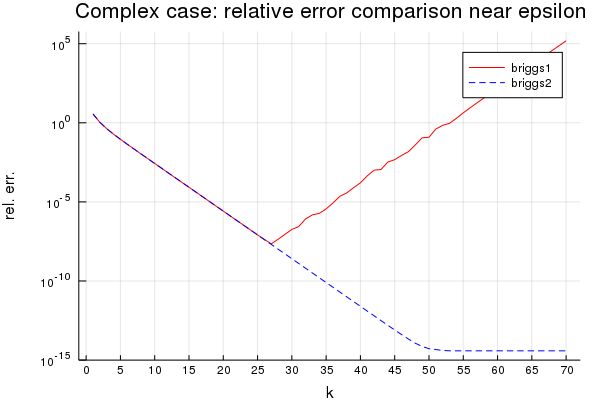
\includegraphics[scale=0.6]{exp2.png}
		\caption{Błąd względny obu algorytmów dla liczb zespolonych i rosnących k}
		\label{fig:exp2}
		\end{figure}

Wykres \ref{fig:exp2} informuje nas o bardzo ważnej własności algorytmu \ref{A:alg1} -- istenieje pewna graniczna wartość $k$, dla której każda kolejna iteracja coraz bardziej oddala nas od dokładnego wyniku. Co więcej, algorytm \ref{A:alg1} jest w stanie obliczyć nie więcej połowę poprawnych cyfr znaczących w porównaniu do algorytmu \ref{A:alg2}.
	
\pagebreak
	\subsection{Eksperyment 3 - błędy względne algorytmów dla precyzji 256-bitowej i zmiennych rzeczywistych.}
	Eksperyment 3 ilustruje zachowanie obu algorytmów na zmiennych rzeczywistych z zakresów odpowiednio $[10^{-16},10^{2}, 10^16]$ na 100 próbkach i $k$=200. Zakresy zostały dobrane tak, aby przetestować działanie na wartościach bardzo małych, średnich i bardzo dużych. 
	
	\begin{figure}[h]
	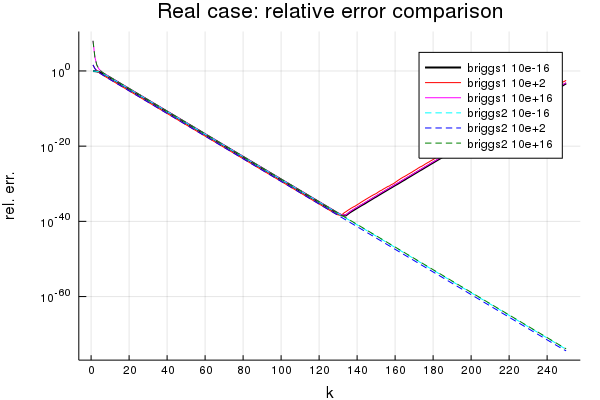
\includegraphics[scale=0.6]{exp3.png}
	\caption{Błąd względny obu algorytmów dla liczb rzeczywistych w arytmetyce wysokiej precyzji}
	\label{fig:exp3}
	\end{figure}

Znów widać przewagę algorytmu \ref{A:alg2}. Przy czterokrotnym zwiększeniu precyzji algorytm \ref{A:alg1} zwiększył swoją dokładność około czterokrotnie, z kolei algorytm \ref{A:alg2} -- ponad $5,5$--krotnie (przez dokładność rozumiemy ilość poprawnych znaczących cyfr dziesiętnych). 

Z wykresu można też wywnioskować, że obie metody nie wymagają odpowiedniego dobierania liczby iteracji $k$ w zależności od argumentu $x$. Oba algorytmy posiadają tę samą właściwość: zarówno dla dużych jak i małych argumentów rząd błędu względnego dla ustalonych $k$ jest taki sam.

\pagebreak
	\subsection{Eksperyment 4 - monotoniczność wartości błędu względnego algorytmu \ref{A:alg2} dla dużych $\mathrm{k}$ i argumentów z $\Re$.}
	Ostatni eksperyment prezentuje zbieżność algorytmu \ref{A:alg2} dla dużych $k$ i stabilność metody liczenia logarytmu za pomocą ulepszonej metody Briggsa.

	\begin{figure}[h]
	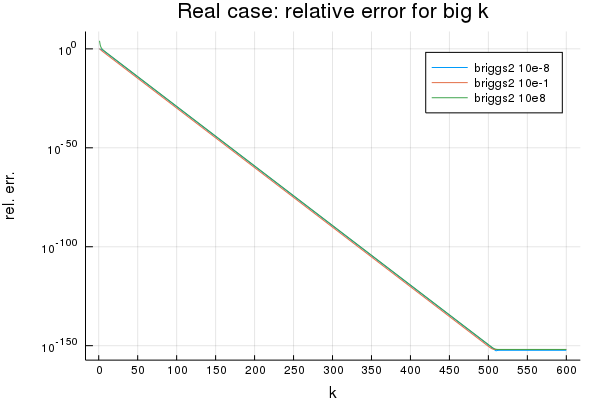
\includegraphics[scale=0.6]{exp4.png}
	\caption{Błąd względny obu algorytmów dla liczb rzeczywistych w arytmetyce wysokiej precyzji}
	\label{fig:exp4}
	\end{figure}
	
	Obliczenia wykonywane zostały na liczbach typu BigFloat o precyzji 512 bitów. Z danych na wykresie \ref{fig:exp4} wynika, że algorytm 2 jest zbieżny w tempie liniowym. Co więcej, zaletą drugiej wersji algorytmu jest jego zachowanie dla bardzo dużych k: kolejne przybliżenia po osiągnięciu granicznej dokładności nie powodują utraty dotychczasowego przybliżenia, jak miało to miejsce w wypadku algorytmu 2.

\pagebreak
\section{Wnioski}
	W arytmetyce zmiennopozycyjnej pewne matematycznie równoznaczne wyrażenia mogą nie być numerycznie tożsame. W związku z tym różne matematyczne sformułowania tego samego problemu mogą skutkować mniej lub bardziej dokładnymi i stabilnymi algorytmami numerycznymi. \\
\indent
	Metoda zaprezentowana przez Awada H. Al-Mohy-ego wykazuje się dużą dokładnością i odpornością na błędy numeryczne. W przeciwieństwie do oryginalnej metody z każdą iteracją produkuje nie gorsze przybliżenia. Dużymi zaletami algorytmu są jego poprawność dla liczb zespolonych, liniowa asymptotyczna złożoność(zakładając stały czas wyznaczania pierwiastka i mnożenia liczb zespolonych) oraz prostota implementacji. Wadą może być natomiast konieczność liczenia pierwiastka, który nieoptymalnie zaimplementowany może mocno zaburzać wynik. Należy pamiętać, że o ile udoskonalony algorytm pozwala na uniknięcie problemu utraty cyfr znaczących przy odejmowaniu, to nie rozwiązuje on problemu złego uwarunkowania zadania w pobliżu punktu $(1+0i)$, gdyż jest to cecha zadania, a nie metody. Co więcej do dziedziny algorytmu nie należą liczby leżące na ujemnej półosi rzeczywistej, więc aby obliczyć wartości funkcji $\log(z)$ dla całej płaszczyzny zespolonej trzeba posiłkować się innymi metodami: algorytm Feynmana, rozwinięcie w szereg funkcji $artanh (z)$, przybliżanie za pomocą średnich arytmetycznych i geometrycznych, przybliżanie za pomocą szeregu harmonicznego i stałej Eulera-Mascheroniego lun innych. Algorytm sprawdza się natomiast bardzo dobrze dla dodatnich liczb rzeczywistych --- najczęściej wykorzystywanych wartości.
	
\begin{thebibliography}{9}
    
\bibitem{al-mohy11} Awad H. Al-Mohy,
\emph{A more accurate Briggs method for the logarithm},
Numerical Algorithms (2011), w druku,
DOI: 10.1007/s11075-011-9496-z.
    
\end{thebibliography}
\end{document}